Eventhough dielectric membranes present a promising platform for doing quantum optomechanics, there is a well known problem in such resonators, namely the fact that they strongly depend of how the silicon frame is clamped \cite{wilson2009}. Clamping the frame is sure to descent the exceptional mechanical properties, because of an increased coupling to the enviroment. Cryogenics is an important tool in realizing a quantum regime enabled system. To establish a heat flow thermal contact and pressure is indeed needed and thereby clamping, as the heat flow is proportional to the cross sectional area between the surfaces \cite{schroeder2000}. One method for suppressing dissipation from the membrane to the frame, is a phononic bandgap shield integrated on the membrane chip \cite{yu2014, tsaturyan2014}.

\begin{figure}[H]
\centering
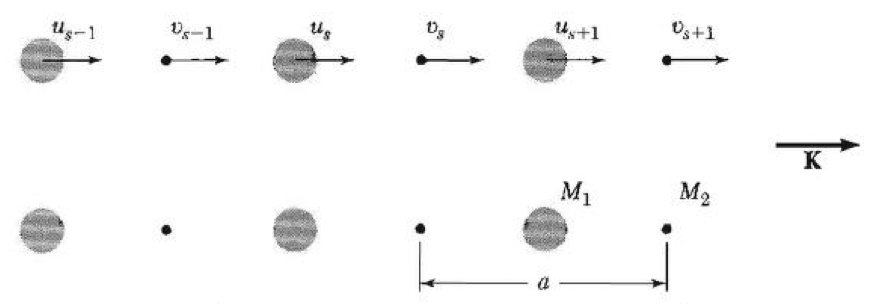
\includegraphics[scale=0.9]{atomic_chain.png}
\caption{Diatomic crystal structure showed in equilibrium positions with masses $M_1$ and $M_2$. The masses are connected to nearest neighbour by a spring constant C in the plane orthogonal to $K$. The atoms displacement of $M_1$ is denoted by $u_{s-1}$, $u_{s}$ and $u_{s+1}$ and $M_2$ by $\nu_{s-1}$, $\nu_{s}$ and $\nu_{s+1}$. The repeated distance is $a$ in the direction of wavevector $K$. Picture is lent from \cite{kittel2005}.}
\label{atomic_chain}
\end{figure}

A phononic bandgap can easily be modelled by an infinite 1D chain of diatomic crystal structure as illustrated in figure \ref{atomic_chain} with two atoms per unit cell \cite{kittel2005}. To see how we construct a basic bandgap we start by writing the equations of motion of such a system

\begin{align}
M_1\frac{d^2u_s}{dt^2} &= C\left( v_s + v_{s-1} - 2u_s \right) \\
M_2\frac{d^2v_s}{dt^2} &= C\left( u_s + u_{s+1} - 2v_s \right).
\end{align}
\noindent
Assuming plane wave solutions

\begin{align}
u_s &= ue^{isKa - i\omega t} \\
v_s &= ve^{isKa - i\omega t}.
\end{align}

we can solve these equation exactly for $\omega^2$. The corresponding dispersion relation can be seen in figure \ref{fig:bandgap}. We examine the limiting case at the upper boundary of the Brillouin zone, where $Ka = \pm \pi$ and find simple relations for the two branches in figure \ref{fig:bandgap}

\begin{align}
\omega_{acu}^2 & = \frac{2C}{M1} \\
\omega_{opt}^2 & = \frac{2C}{M2}.
\end{align}
\noindent
We can from these relations see that the size of the bandgap depends on ratio of the two masses.

\begin{figure}[H]
\centering
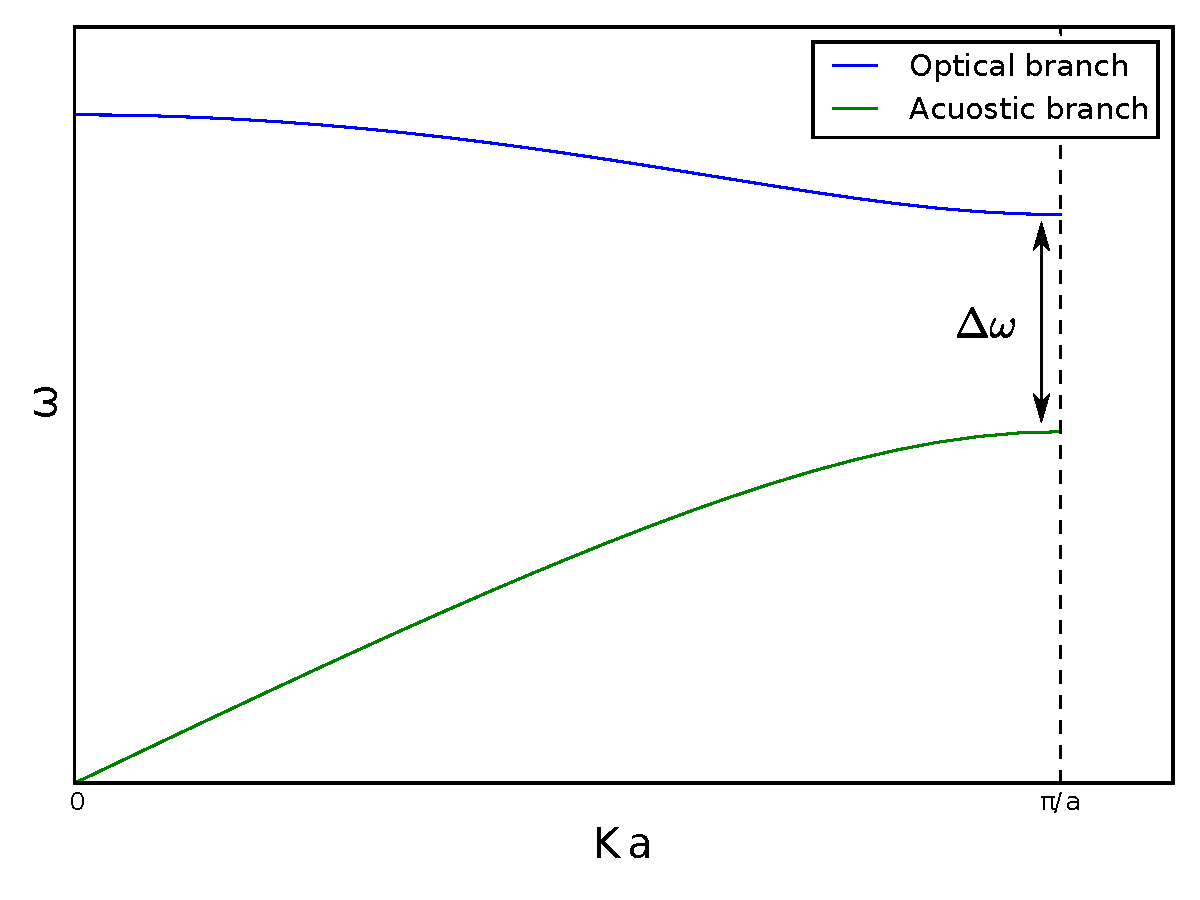
\includegraphics[scale=0.5]{bandgap.pdf}
\caption{Bands plotted for longitudinal modes. We see that we get a bandgap $\Delta\omega$ where no propagating modes can exist.}
\label{fig:bandgap}
\end{figure}

Calculating the dispersion relation of a real structure is however done numerically\footnote{Simulations are done using COMSOL Multiphysics by Yeghishe Tsaturyan. COMSOL is a commercial finite element analysis software.} and the resulting dispersion is, see figure \ref{fig:simulated_bandgap}.

\begin{figure}[H]
\centering
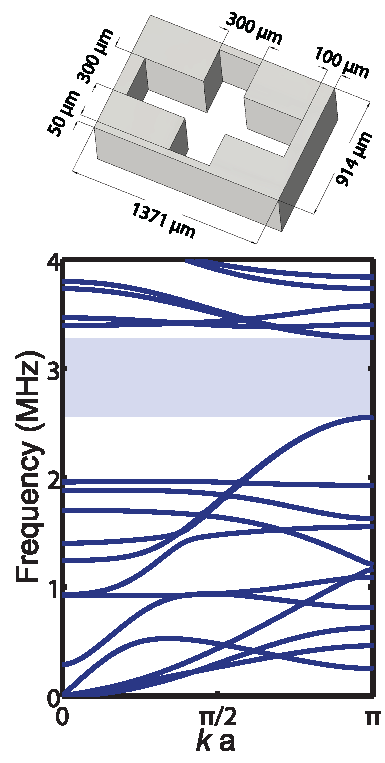
\includegraphics[scale=0.6]{bandgapery.pdf}
\caption{COMSOL simulated phononic structure \cite{tsaturyan2014}.}
\label{fig:simulated_bandgap}
\end{figure}
\noindent
To relate figure \ref{atomic_chain} to the actual structure in figure \ref{fig:simulated_bandgap}, see figure \ref{fig:spring_mass}.

\begin{figure}[H]
\centering
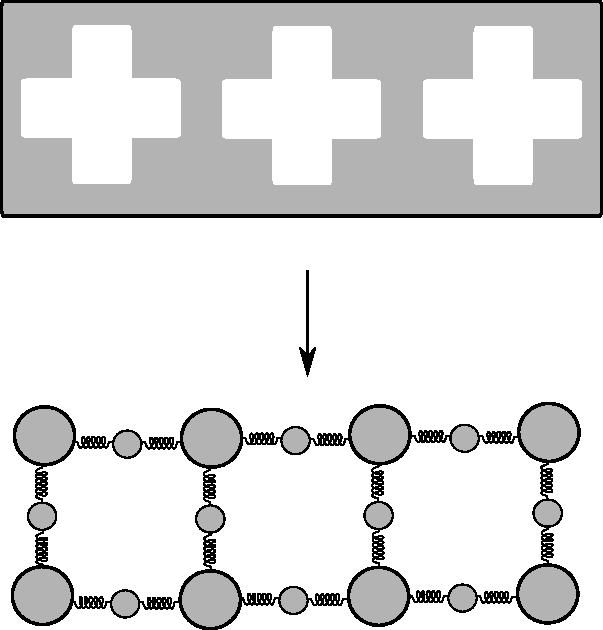
\includegraphics[scale=0.5]{spring_mass.pdf}
\caption{Our phononic structure ``translated" into the diatomic crystal model.}
\label{fig:spring_mass}
\end{figure}